\chapter{METODE PENELITIAN}
\section{Tempat dan Waktu Penelitian}
Penelitian ini dilaksanakan dari bulan Februari 2025 hingga Juni
2025, bertempat di Laboratorium Elektronika dan Instrumentasi,
Departemen Fisika, Fakultas Matematika dan Ilmu Pengetahuan Alam,
Universitas Hasanuddin, Makassar.

\vspace{1em}

\section{Peralatan Penelitian}
Adapun peralatan yang digunakan pada penelitian ini adalah sebagai berikut:
\begin{enumerate}
  \item Arduino Uno berfungsi sebagai mikrokontroler utama yang
    mengendalikan motor \textit{servo} pada lengan robot serta menerima sinyal
    dari sensor.
  \item Motor \textit{servo} digunakan sebagai aktuator untuk menggerakkan
    bagian-bagian lengan robot sesuai perintah dari Arduino.
  \item Lengan robot EEZYbotARM MK1 berfungsi sebagai struktur
    mekanik yang menjadi tempat pemasangan motor \textit{servo} dan berperan
    sebagai sistem pergerakan robotik.
  \item \textit{Power supply} 5V berfungsi memberikan catu daya stabil untuk
    motor \textit{servo} agar dapat beroperasi dengan baik.
  \item \textit{Sensor Passive Infrared Receiver} (PIR) HC-SR501
    digunakan untuk mendeteksi gerakan dan membantu
    menghitung jumlah kontainer cacat dan non-cacat yang lewat.
  \item Kamera digunakan untuk mengambil gambar kontainer kimia, yang
    kemudian diproses oleh model deteksi (YOLO) dan deteksi cacat
    (\textit{autoencoder}).
  \item Laptop/komputer digunakan untuk mengunggah program ke Arduino
    Uno, serta menjalankan model deteksi berbasis YOLO dan
    \textit{autoencoder} untuk analisis visual.
  \item Kabel \textit{jumper} berfungsi menghubungkan berbagai komponen
    elektronik seperti sensor dan aktuator ke papan rangkaian dan
    Arduino.
  \item Papan rangkaian berfungsi untuk menyediakan jalur koneksi
    antar komponen.
\end{enumerate}

\vspace{1em}

\section{Metode Kerja}
Dalam penelitian ini terdapat beberapa tahapan yang harus dilakukan.
Tahapan penelitian secara lengkap dapat dilihat pada bagan alir yang
tertera pada Gambar \ref{fig:bagan-umum}. Penelitian ini dibatasi
pada perancangan dan pembuatan prototipe sistem deteksi cacat otomatis.

% \begin{figure}[H]
%   \centering
%   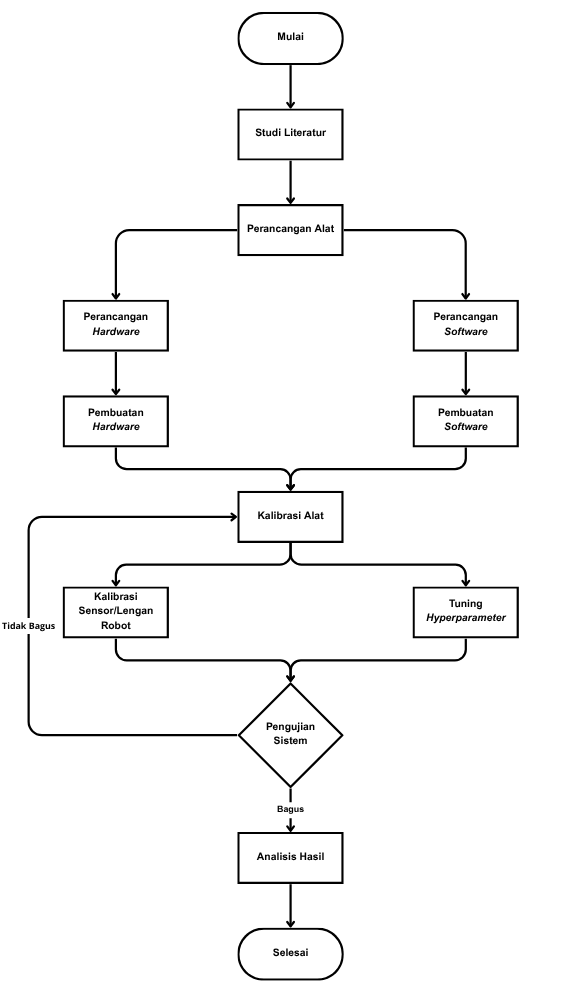
\includegraphics[width=0.7\textwidth]{gambar/bagan-umum.png}
%   \caption{Bagan alir penelitian}
%   \label{fig:bagan-umum}
% \end{figure}
% \vspace{-1em}

\begin{figure}[H]
  \centering
  \begin{tikzpicture}[
      every node/.style={font=\fontsize{9}{11}\selectfont},
      node distance = 0.77cm and 1cm
    ]
    \node (mulai) [startstop] {Mulai};
    \node (literatur) [process, below=of mulai] {Studi Literatur};
    \node (perancangan-alat) [process, below=of literatur] {Perancangan Alat};
    \node (perancangan-hardware) [process, align=center, below
    left=of perancangan-alat]
    {Perancangan \\ \textit{Hardware}};
    \node (perancangan-software) [process, align=center, below
    right=of perancangan-alat]
    {Perancangan \\ \textit{Software}};
    \node (pembuatan-hardware) [process, align=center, below=of
    perancangan-hardware]
    {Pembuatan \\ \textit{Hardware}};
    \node (pembuatan-software) [process, align=center, below=of
    perancangan-software]
    {Pembuatan \\ \textit{Software}};
    \coordinate (merge1) at
    ($(pembuatan-hardware.south)!0.5!(pembuatan-software.south)$);
    \node (kalibrasi-alat) [process, align=center, below=of merge1,
    yshift=-0.5cm] {Kalibrasi Alat};
    \node (kalibrasi-sensor) [process, align=center, below left=of
    kalibrasi-alat]
    {Kalibrasi \\ Sensor/Lengan Robot};
    \node (kalibrasi-parameter) [process, align=center, below
    right=of kalibrasi-alat]
    {\textit{Tuning} \\ \textit{Hyperparameter}};
    \coordinate (merge2) at
    ($(kalibrasi-sensor.south)!0.5!(kalibrasi-parameter.south)$);
    \node (pengujian-sistem) [decision, align=center, below=of
    merge2, yshift=-0.5cm] {Pengujian \\ Sistem};
    \node (analisis-hasil) [process, below=of pengujian-sistem]
    {Analisis Hasil};
    \node (selesai) [startstop, below=of analisis-hasil]
    {Selesai};

    % Arrow
    \draw [arrow] (mulai) -- (literatur);
    \draw [arrow] (literatur) -- (perancangan-alat);

    \draw [arrow] (perancangan-alat.west) -| (perancangan-hardware.north);
    \draw [arrow] (perancangan-alat.east) -| (perancangan-software.north);
    \draw [arrow] (perancangan-hardware) -- (pembuatan-hardware);
    \draw [arrow] (perancangan-software) -- (pembuatan-software);

    \draw [arrow] (pembuatan-hardware.south) --
    ($(pembuatan-hardware.south)+(0,-0.67cm)$) -| (kalibrasi-alat.north);
    \draw [arrow] (pembuatan-software.south) --
    ($(pembuatan-software.south)+(0,-0.67cm)$) -| (kalibrasi-alat.north);

    \draw [arrow] (kalibrasi-alat.south) --
    ($(kalibrasi-alat.south)+(0,-0.35cm)$) -| (kalibrasi-sensor.north);
    \draw [arrow] (kalibrasi-alat.south) --
    ($(kalibrasi-alat.south)+(0,-0.35cm)$) -| (kalibrasi-parameter.north);

    \draw [arrow] (kalibrasi-sensor.south) --
    ($(kalibrasi-sensor.south)+(0,-0.6cm)$) -| (pengujian-sistem.north);
    \draw [arrow] (kalibrasi-parameter.south) --
    ($(kalibrasi-parameter.south)+(0,-0.6cm)$) -| (pengujian-sistem.north);

    \draw [arrow] (pengujian-sistem.west) -- node[midway,
    yshift=0.25cm]{Tidak Bagus}
    ($(pengujian-sistem.west)+(-4.7cm,0)$) |- (kalibrasi-alat.west);
    \draw [arrow] (pengujian-sistem) -- node[midway, xshift=0.5cm]{Bagus}
    (analisis-hasil);

    \draw [arrow] (analisis-hasil) -- (selesai);

  \end{tikzpicture}
  \caption{Bagan alir penelitian}
  \label{fig:bagan-umum}
\end{figure}
\vspace{-1em}

Tahapan dimulai dengan kajian mendalam terhadap teknologi robotik,
algoritma \textit{autoencoder} untuk deteksi anomali visual, serta
metode deteksi objek seperti (YOLO).
Setelah pemahaman awal diperoleh, dilakukan
perancangan sistem yang mencakup perangkat keras (lengan robot dan
sensor) serta perangkat lunak berupa algoritma \textit{machine
learning}. Selanjutnya, sistem robot dikalibrasi agar dapat bekerja
secara optimal, termasuk proses \textit{tuning hyperparameter} pada
model \textit{machine learning}. Jika sistem telah berfungsi sesuai
dengan yang diharapkan, maka dilanjutkan dengan proses pengambilan data
sebagai langkah awal dalam pengujian dan validasi model.

\vspace{1em}

\subsection{Perancangan \textit{Hardware}}
Penelitian ini dimulai dengan tahap perancangan \textit{hardware}. Komponen
\textit{hardware} meliputi kamera untuk mengambil gambar
kontainer kimia, laptop sebagai pusat pemrosesan dan eksekusi
algoritma \textit{machine learning}, serta sensor PIR untuk menghitung
jumlah kontainer kimia. Adapun
rancangan \textit{hardware} dapat dilihat pada Gambar \ref{fig:rangkaian}.

\begin{figure}[H]
  \centering
  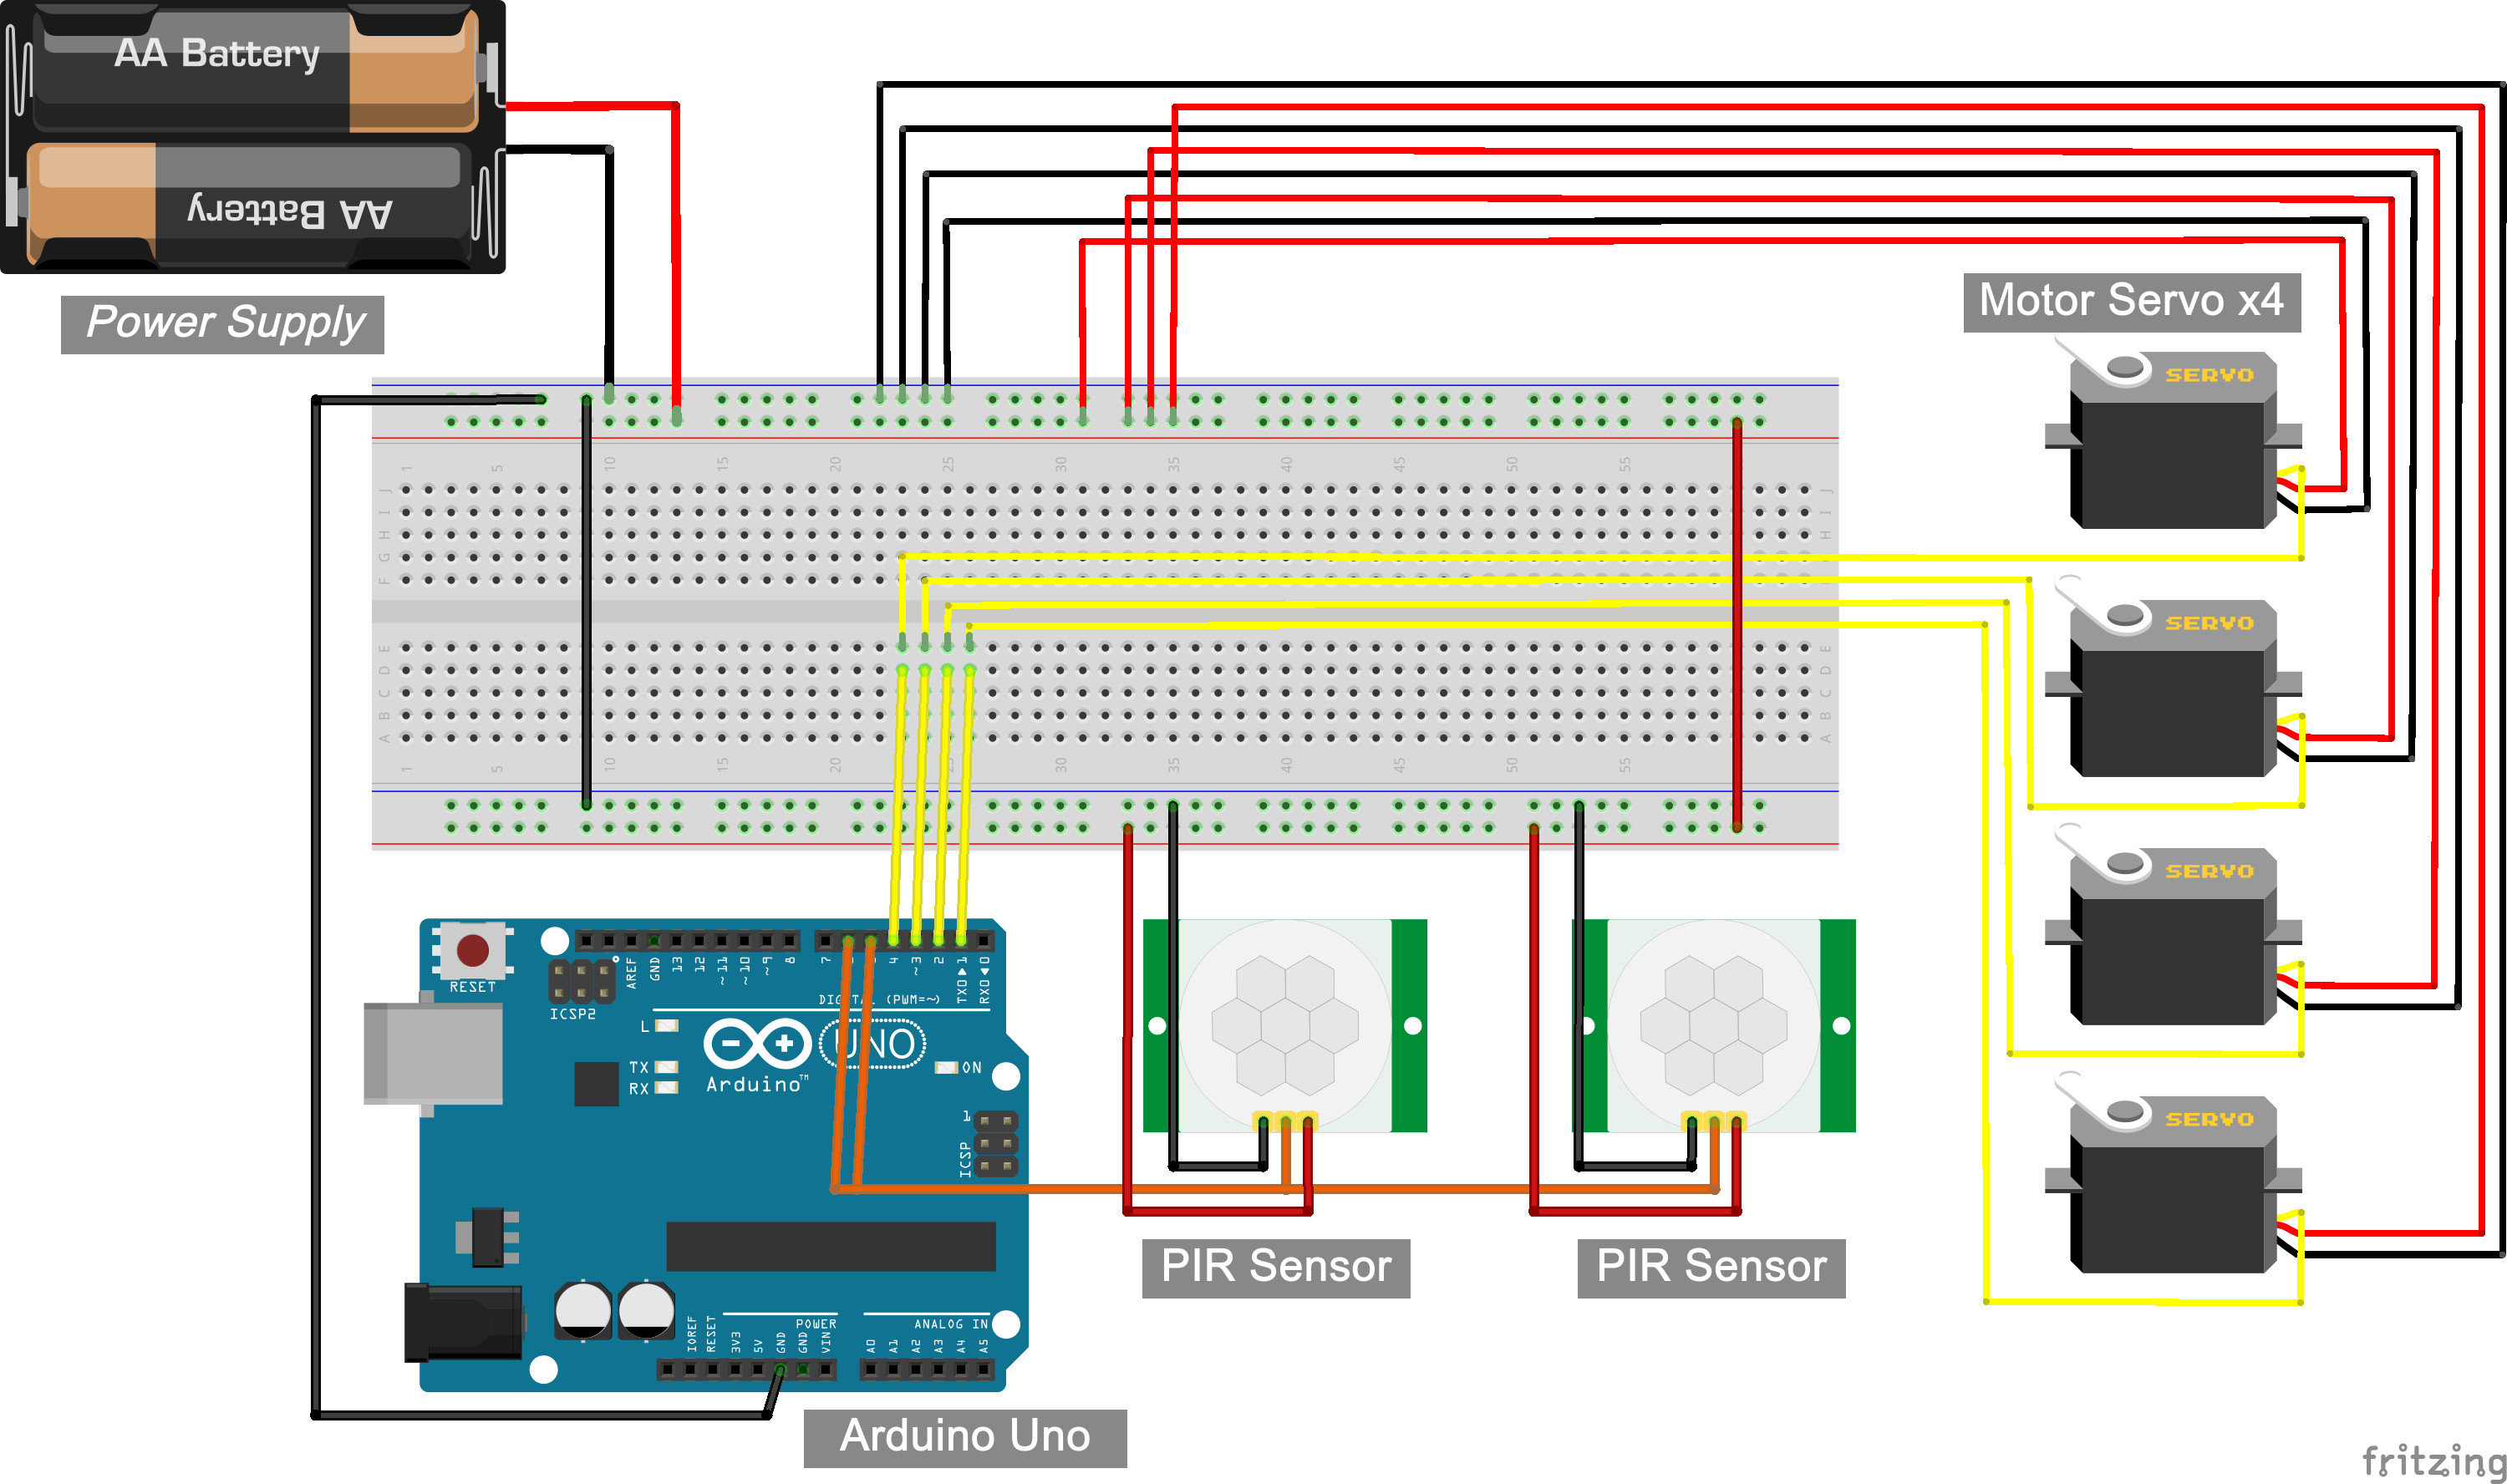
\includegraphics[width=\textwidth]{gambar/rangkaian.jpg}
  \caption{Rangkaian \textit{hardware} sistem}
  \label{fig:rangkaian}
\end{figure}
\vspace{-1em}

Sistem diawali saat kamera menangkap gambar kontainer kimia yang
diletakkan di area pengambilan gambar. Gambar ini diproses oleh model
deteksi objek (YOLO) untuk mengenali keberadaan kontainer sebelum
tahap deteksi cacat. Selanjutnya, gambar yang telah dikenal dikirim
ke model deteksi kecacatan berbasis \textit{convolutional variational
autoencoder} (CVAE) untuk
menentukan apakah kontainer mengalami cacat atau tidak. Berdasarkan
hasil prediksi tersebut, sinyal dikirim ke Arduino
untuk menggerakkan \textit{servo} sebagai respon terhadap kondisi
kontainer. Lengan robot kemudian mengambil kontainer kimia dan memindahkannya ke
wadah yang sesuai, tergantung pada hasil deteksi. Untuk memantau dan
menghitung jumlah
kontainer yang telah dipindahkan, dua sensor PIR dipasang pada
masing-masing wadah (cacat dan tidak). Data dari sensor ini
dikirim ke \textit{web server}, yang menyediakan API untuk dikonsumsi
agar data jumlah kontainer dapat ditampilkan ke klien secara
\textit{real-time}. Secara keseluruhan, keterkaitan antar komponen
perangkat keras dalam sistem ini dapat dilihat pada Gambar \ref{fig:hardware}.

\begin{figure}[H]
  \centering
  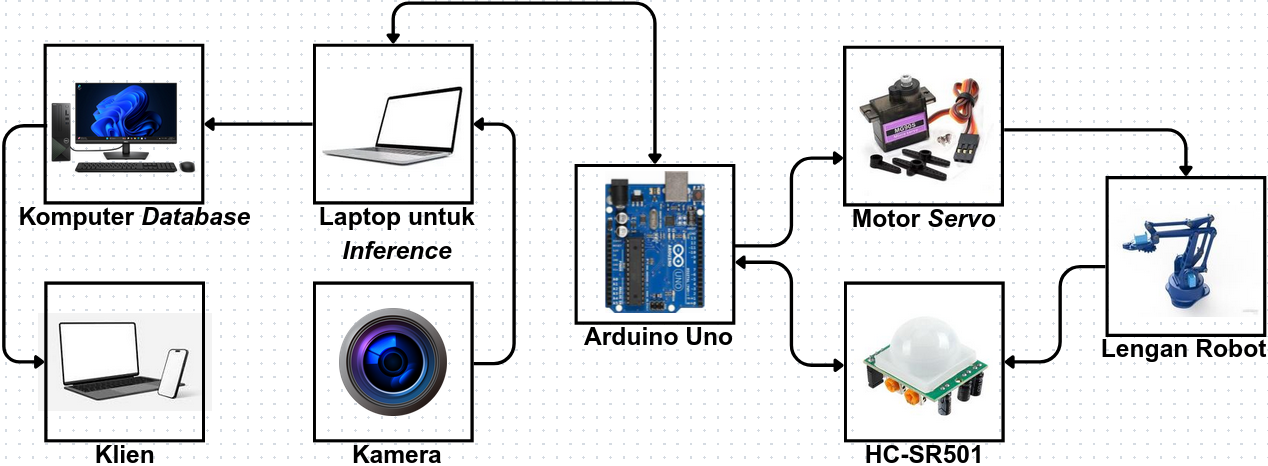
\includegraphics[width=\textwidth]{gambar/rancang.png}
  \caption{Rancang sistem \textit{hardware}}
  \label{fig:hardware}
\end{figure}
\vspace{-1em}

\vspace{1em}

\subsection{Perancangan \textit{Software}}
Perangkat lunak mencakup perancangan beberapa
algoritma inti. Pertama, dirancang model deteksi objek berbasis YOLO
untuk mengenali kontainer kimia pada citra yang diambil oleh kamera.
Kedua, digunakan CVAE sebagai model untuk
mendeteksi cacat kontainer. Selain itu,
juga dirancang algoritma kontrol untuk mengatur pergerakan lengan
robot dalam mengambil dan memindahkan kontainer berdasarkan hasil
klasifikasi. Sistem ini juga terintegrasi dengan modul
\textit{Internet of Things} (IoT) untuk menampilkan data kontainer
cacat dan non-cacat
pada klien secara \textit{real-time} melalui \textit{website}. \par

Tahap perancangan model deteksi objek dimulai dengan pengumpulan
\textit{dataset} berupa gambar kontainer kimia dari berbagai kondisi
dan sudut pandang menggunakan kamera. Setelah gambar terkumpul, dilakukan
proses anotasi dengan memberikan label dan \textit{bounding box} pada
setiap kontainer sesuai dengan format yang dibutuhkan oleh algoritma
YOLO. \textit{Dataset} yang telah dianotasi digunakan untuk
melatih model. Setelah proses pelatihan selesai, model dievaluasi
menggunakan data uji yang belum pernah dilihat sebelumnya. Evaluasi
dilakukan menggunakan beberapa metrik seperti \textit{precision},
\textit{recall}, dan \textit{mean Average Precision} (mAP), guna
memastikan model memiliki kemampuan generalisasi yang baik.
Alur perancangan model deteksi objek dapat dilihat pada
Gambar \ref{fig:pipeline-yolo}.

% \begin{figure}[H]
%   \centering
%   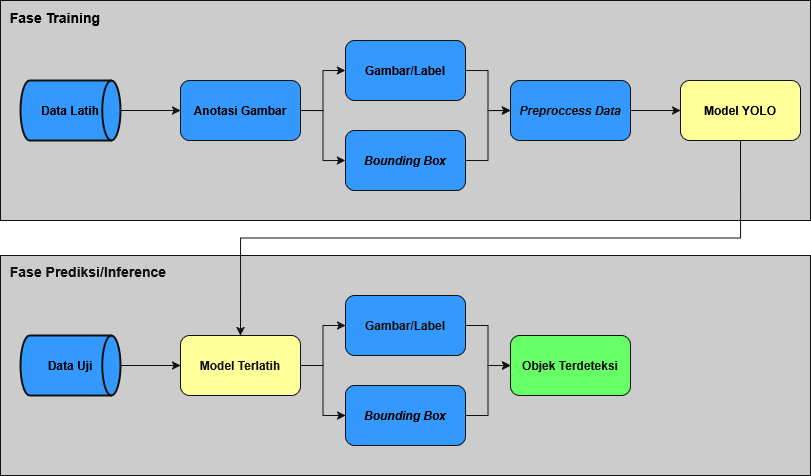
\includegraphics[width=\textwidth]{gambar/pipeline_yolo.png}
%   \caption{Diagram \textit{pipeline} pelatihan model YOLO}
%   \label{fig:pipeline-yolo}
% \end{figure}
% \vspace{-1em}

\begin{figure}[H]
  \centering
  \begin{tikzpicture}[
      every node/.style={font=\fontsize{8.5}{11}\selectfont},
      node distance = 0.5cm and 0.5cm
    ]
    % --- Pipeline pertama ---
    \node (data-latih1) [data] {Data Latih};
    \node (anotasi1) [pipeline-box, fill=cyan!50, right=of
    data-latih1] {Anotasi Gambar};
    \node (gambar-label1) [pipeline-box, fill=cyan!50, above right=of
    anotasi1] {Gambar/Label};
    \node (bounding-box1) [pipeline-box, fill=cyan!50, below right=of
    anotasi1] {\textit{Bounding Box}};
    \node (preprocess1) [pipeline-box, fill=cyan!50, above right=of
    bounding-box1] {\textit{Preprocess Data}};
    \node (yolo1) [pipeline-box, fill=yellow!50, right=of
    preprocess1] {Model Yolo};

    % Node dummy
    \node (start-bawah) [below=3cm of data-latih1] {};

    % --- Pipeline kedua ---
    \node (data-uji) [data, below=of start-bawah, xshift=1cm] {Data Uji};
    \node (model-terlatih) [pipeline-box, fill=yellow!50, right=of
    data-uji] {Model Terlatih};
    \node (gambar-label2) [pipeline-box, fill=cyan!50, above right=of
    model-terlatih] {Gambar/Label};
    \node (bounding-box2) [pipeline-box, fill=cyan!50, below right=of
    model-terlatih] {\textit{Bounding Box}};
    \node (objek-terdeteksi) [pipeline-box, fill=green!50, above
    right=of bounding-box2] {Objek Terdeteksi};

    % Arrow
    \draw [arrow] (data-latih1) -- (anotasi1);
    \draw [arrow] (anotasi1.east) -- ($(anotasi1.east)+(0.25cm, 0)$)
    |- (gambar-label1);
    \draw [arrow] (anotasi1.east) -- ($(anotasi1.east)+(0.25cm, 0)$)
    |- (bounding-box1);
    \draw [arrow] (gambar-label1.east) -- ($(gambar-label1.east)+(0.20cm, 0)$)
    |- (preprocess1);
    \draw [arrow] (bounding-box1.east) -- ($(bounding-box1.east)+(0.20cm, 0)$)
    |- (preprocess1);
    \draw [arrow] (preprocess1) -- (yolo1);

    \draw [arrow] (data-uji) -- (model-terlatih);
    \draw [arrow] (model-terlatih.east) -- ($(model-terlatih.east)+(0.25cm, 0)$)
    |- (gambar-label2);
    \draw [arrow] (model-terlatih.east) -- ($(model-terlatih.east)+(0.25cm, 0)$)
    |- (bounding-box2);
    \draw [arrow] (gambar-label2.east) -- ($(gambar-label2.east)+(0.20cm, 0)$)
    |- (objek-terdeteksi);
    \draw [arrow] (bounding-box2.east) -- ($(bounding-box2.east)+(0.20cm, 0)$)
    |- (objek-terdeteksi);

    \draw [arrow] (yolo1.south) -- ($(yolo1.south)+(0,-1.9cm)$) -| (data-uji);
  \end{tikzpicture}
  \caption{Diagram alur pelatihan model YOLO}
  \label{fig:pipeline-yolo}
\end{figure}
\vspace{-1em}

Berikutnya adalah tahap pembangunan model deteksi cacat menggunakan
algoritma CVAE. Tahap ini menggunakan
\textit{dataset} yang sama seperti pada pelatihan model YOLO dengan
beberapa tambahan, namun tanpa menggunakan anotasi \textit{bounding
box} karena sifat \textit{unsupervised} dari \textit{autoencoder}.
Data diproses melalui tahap \textit{preprocessing} seperti
mengubah dimensi gambar, normalisasi, dan augmentasi untuk
meningkatkan variasi. Model
dirancang dengan dua komponen utama: \textit{encoder} untuk
mengekstraksi fitur penting dan menghasilkan representasi berdimensi
rendah (ruang laten), serta \textit{decoder} untuk
merekonstruksi gambar dari representasi tersebut. Setelah arsitektur
selesai dan data siap, model dilatih untuk meminimalkan perbedaan
antara gambar asli dan hasil rekonstruksi, sehingga mampu mengenali
citra normal secara akurat. Evaluasi dilakukan dengan menghitung
\textit{reconstruction error}, yang digunakan untuk membedakan antara
gambar normal dan cacat. Ambang batas deteksi ditentukan melalui analisis
distribusi \textit{error} pada data validasi. Alur perancangan model
deteksi cacat dapat dilihat pada Gambar \ref{fig:pipeline-autoencoder}.

% \begin{figure}[H]
%   \centering
%   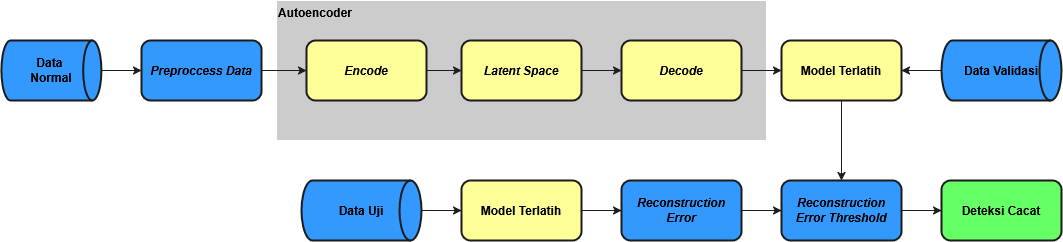
\includegraphics[width=\textwidth]{gambar/pipeline_autoencoder.png}
%   \caption{Diagram \textit{pipeline} pelatihan model deteksi cacat}
%   \label{fig:pipeline-autoencoder}
% \end{figure}
% \vspace{-1em}

\begin{figure}[H]
  \centering
  \begin{tikzpicture}[
      every node/.style={font=\fontsize{9}{11}\selectfont},
      node distance = 1cm and 2cm
    ]
    \node (data-normal) [data] {Data Normal};
    \node (preprocess) [pipeline-box, fill=cyan!50, below=of
    data-normal] {\textit{Preprocess Data}};
    \node (encode) [pipeline-box, fill=yellow!50, below=of
    preprocess] {\textit{Encode}};
    \node (latent-space) [pipeline-box, fill=yellow!50, below=of
    encode] {Ruang Laten};
    \node (decode) [pipeline-box, fill=yellow!50, below=of
    latent-space] {\textit{Decode}};
    \node (model-terlatih) [pipeline-box, fill=yellow!50, below=of
    decode] {Model Terlatih};
    \node (data-validasi) [data, below=of
    model-terlatih] {Data Validasi};

    \node (data-uji) [data, left=of encode] {Data Uji};
    \node (model-terlatih2) [pipeline-box, fill=cyan!50, below=of
    data-uji] {Model Terlatih};
    \node (reconstruction) [pipeline-box, align=center, fill=cyan!50, below=of
    model-terlatih2]
    {\textit{Reconstruction} \\ \textit{Error}};
    \node (threshold) [pipeline-box, align=center, fill=cyan!50, below=of
    reconstruction]
    {\textit{Reconstruction Error} \\ \textit{Threshold}};
    \node (deteksi-cacat) [pipeline-box, fill=green!50, below=of
    threshold] {Deteksi Cacat};

    % Arrow
    \draw [arrow] (data-normal) -- (preprocess);
    \draw [arrow] (preprocess) -- (encode);
    \draw [arrow] (preprocess) -- (encode);
    \draw [arrow] (encode) -- (latent-space);
    \draw [arrow] (latent-space) -- (decode);
    \draw [arrow] (decode) -- (model-terlatih);
    \draw [arrow] (data-validasi) -- (model-terlatih);
    \draw [arrow] (data-uji) -- (model-terlatih2);
    \draw [arrow] (model-terlatih2) -- (reconstruction);
    \draw [arrow] (reconstruction) -- (threshold);
    \draw [arrow] (model-terlatih) -- (threshold);
    \draw [arrow] (threshold) -- (deteksi-cacat);
  \end{tikzpicture}
  \caption{Diagram alur pelatihan model deteksi cacat}
  \label{fig:pipeline-autoencoder}
\end{figure}
\vspace{-1em}

\vspace{1em}

\subsection{Bagan Alir Sistem Kerja Alat}
Bagan alir kerja sistem secara keseluruhan dimulai saat kamera
menangkap citra, yang kemudian diproses oleh model YOLO untuk
mendeteksi objek kontainer. Setelah terdeteksi, model
\textit{autoencoder} menganalisis citra tersebut untuk menentukan
apakah terdapat kecacatan. Terakhir, informasi mengenai hasil
penyortiran dikirimkan ke \textit{web server} untuk keperluan
pemantauan. Perancangan bagan alir sistem kerja alat secara
keseluruhan ditunjukkan pada Gambar \ref{fig:bagan-alir-kerja}.

% \begin{figure}[H]
%   \centering
%   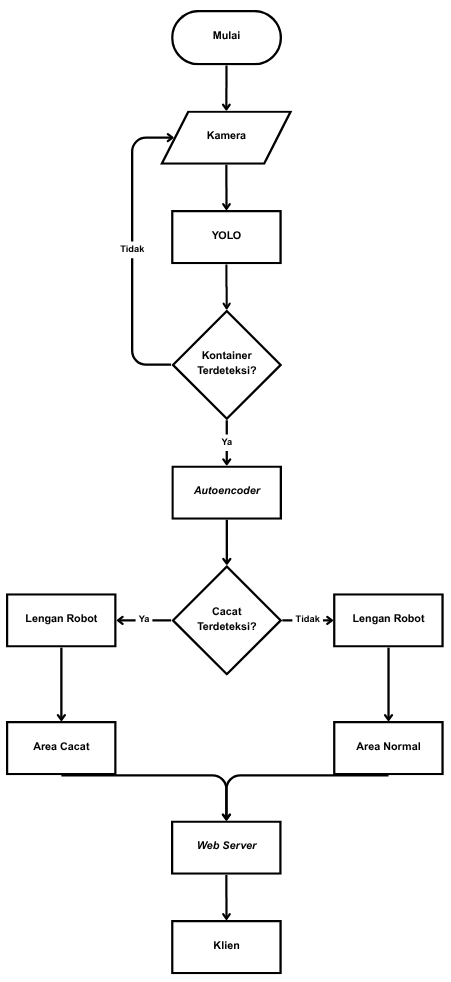
\includegraphics[width=0.7\textwidth]{gambar/flowchart.png}
%   \caption{Bagan alir sistem kerja alat}
%   \label{fig:bagan-alir-kerja}
% \end{figure}
% \vspace{-1em}

\begin{figure}[H]
  \centering

  \begin{tikzpicture}[
      every node/.style={font=\fontsize{9}{11}\selectfont},
      node distance = 0.75cm and 1.5cm
    ]
    \node (mulai) [startstop] {Mulai};
    \node (kamera) [input, below=of mulai] {Kamera};
    \node (yolo) [process, below=of kamera] {YOLO};
    \node (kontainer-terdeteksi) [decision, align=center, below=of yolo]
    {Kontainer \\ Terdeteksi?};
    \node (autoencoder) [process, below=of kontainer-terdeteksi]
    {\textit{Autoencoder}};

    \node (cacat-terdeteksi) [decision, align=center, below=of autoencoder]
    {Cacat \\ Terdeteksi?};
    \node (lengan-cacat) [process, left=of cacat-terdeteksi] {Lengan Robot};
    \node (area-cacat) [process, below=of lengan-cacat] {Area Cacat};
    \node (lengan-normal) [process, right=of cacat-terdeteksi] {Lengan Robot};
    \node (area-normal) [process, below=of lengan-normal] {Area Normal};

    \node (web) [process, below left=of area-normal] {\textit{Web Server}};
    \node (klien) [process, below=of web] {Klien};
    \node (selesai) [startstop, below=of klien] {Selesai};

    % Arrow
    \draw [arrow] (mulai) -- (kamera);
    \draw [arrow] (kamera) -- (yolo);
    \draw [arrow] (yolo) -- (kontainer-terdeteksi);

    \draw [arrow] (kontainer-terdeteksi) -- node[midway,
    xshift=0.3cm]{Iya} (autoencoder);
    \draw [arrow] (kontainer-terdeteksi.west) -- node[midway,
    yshift=0.25cm]{Tidak}
    ($(kontainer-terdeteksi.west)+(-2cm,0)$) |- (kamera.west);

    \draw [arrow] (autoencoder) -- (cacat-terdeteksi);
    \draw [arrow] (cacat-terdeteksi.east) -- node[midway, yshift=0.25cm]{Tidak}
    (lengan-normal);
    \draw [arrow] (cacat-terdeteksi.west) -- node[midway,
    yshift=0.25cm]{Iya} (lengan-cacat);
    \draw [arrow] (lengan-cacat) -- (area-cacat);
    \draw [arrow] (lengan-normal) -- (area-normal);

    \draw [arrow] (area-cacat.south) --
    ($(area-cacat.south)+(0,-0.4)$) -| (web.north);
    \draw [arrow] (area-normal.south) --
    ($(area-normal.south)+(0,-0.4)$) -| (web.north);

    \draw [arrow] (web) -- (klien);
    \draw [arrow] (klien) -- (selesai);

  \end{tikzpicture}
  \caption{Bagan alir sistem kerja alat}
  \label{fig:bagan-alir-kerja}
\end{figure}
\vspace{-1em}
